%!TEX root = thesis.tex

%% appendix.tex
%%

%% ==============================
%\chapter{Appendix}
%\label{ch:Appendix}
%% ==============================

\appendix

\iflanguage{english}
{\addchap{Appendix}}	% english style
{\addchap{Anhang}}	% german style

\section{Introduction}
\begin{figure}
  \centering
  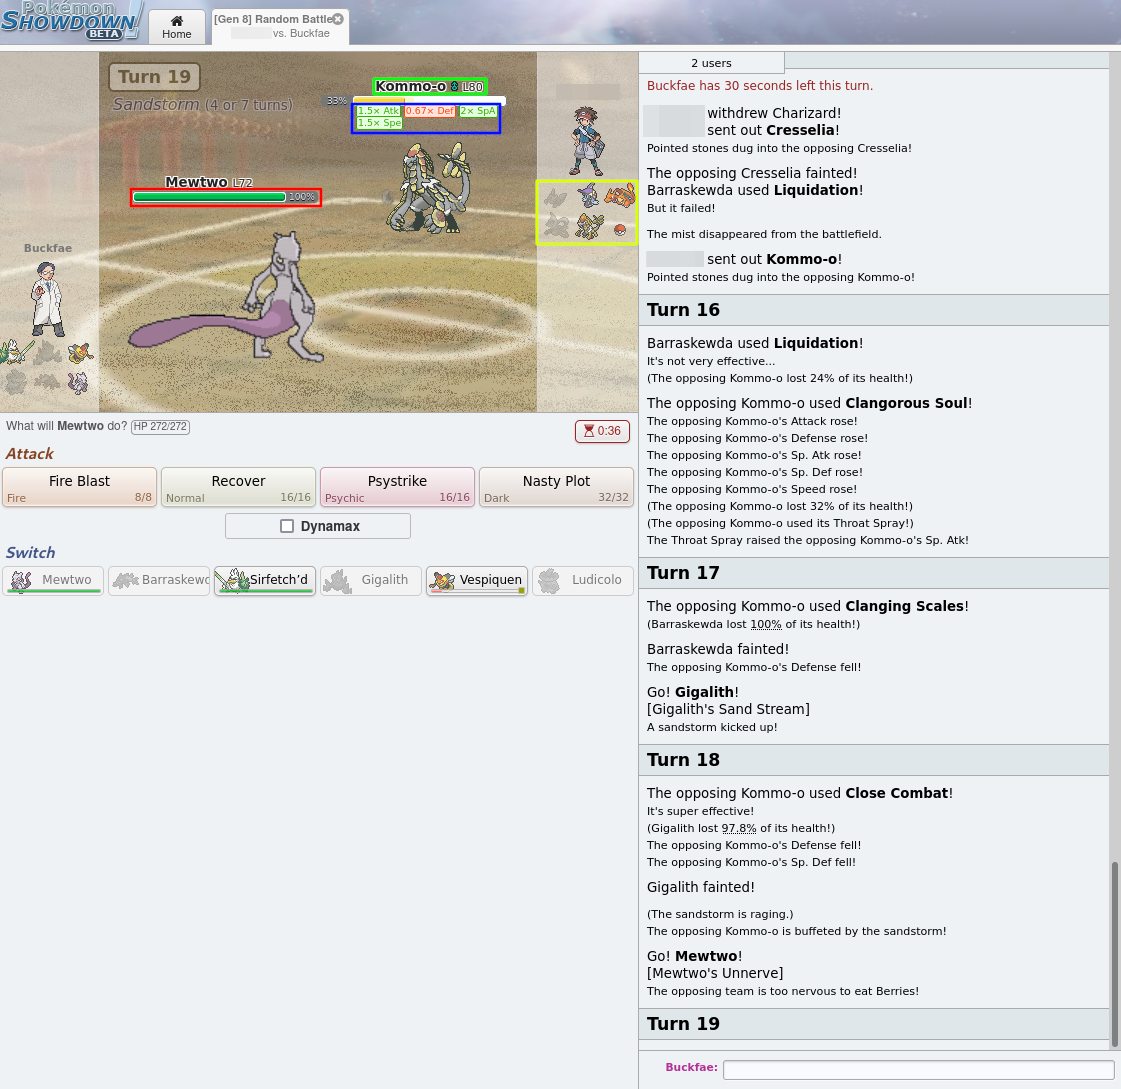
\includegraphics[width=1\textwidth]{images/Showdown.png}
  \caption{Battle between two players on \textit{Pokémon Showdown}. The \textit{Mewtwo} of the player \textit{Buckfae} is at full
  health while the opposing \textit{Kommo-o} has 33\% of his health remaining. Below the game window, all possible actions
  for the player is displayed. A log of previous actions is displayed on the right-hand side.}
  \label{fig:showdown-battle}
\end{figure}

\section{Related Work}
\begin{sidewaysfigure}
	\centering
	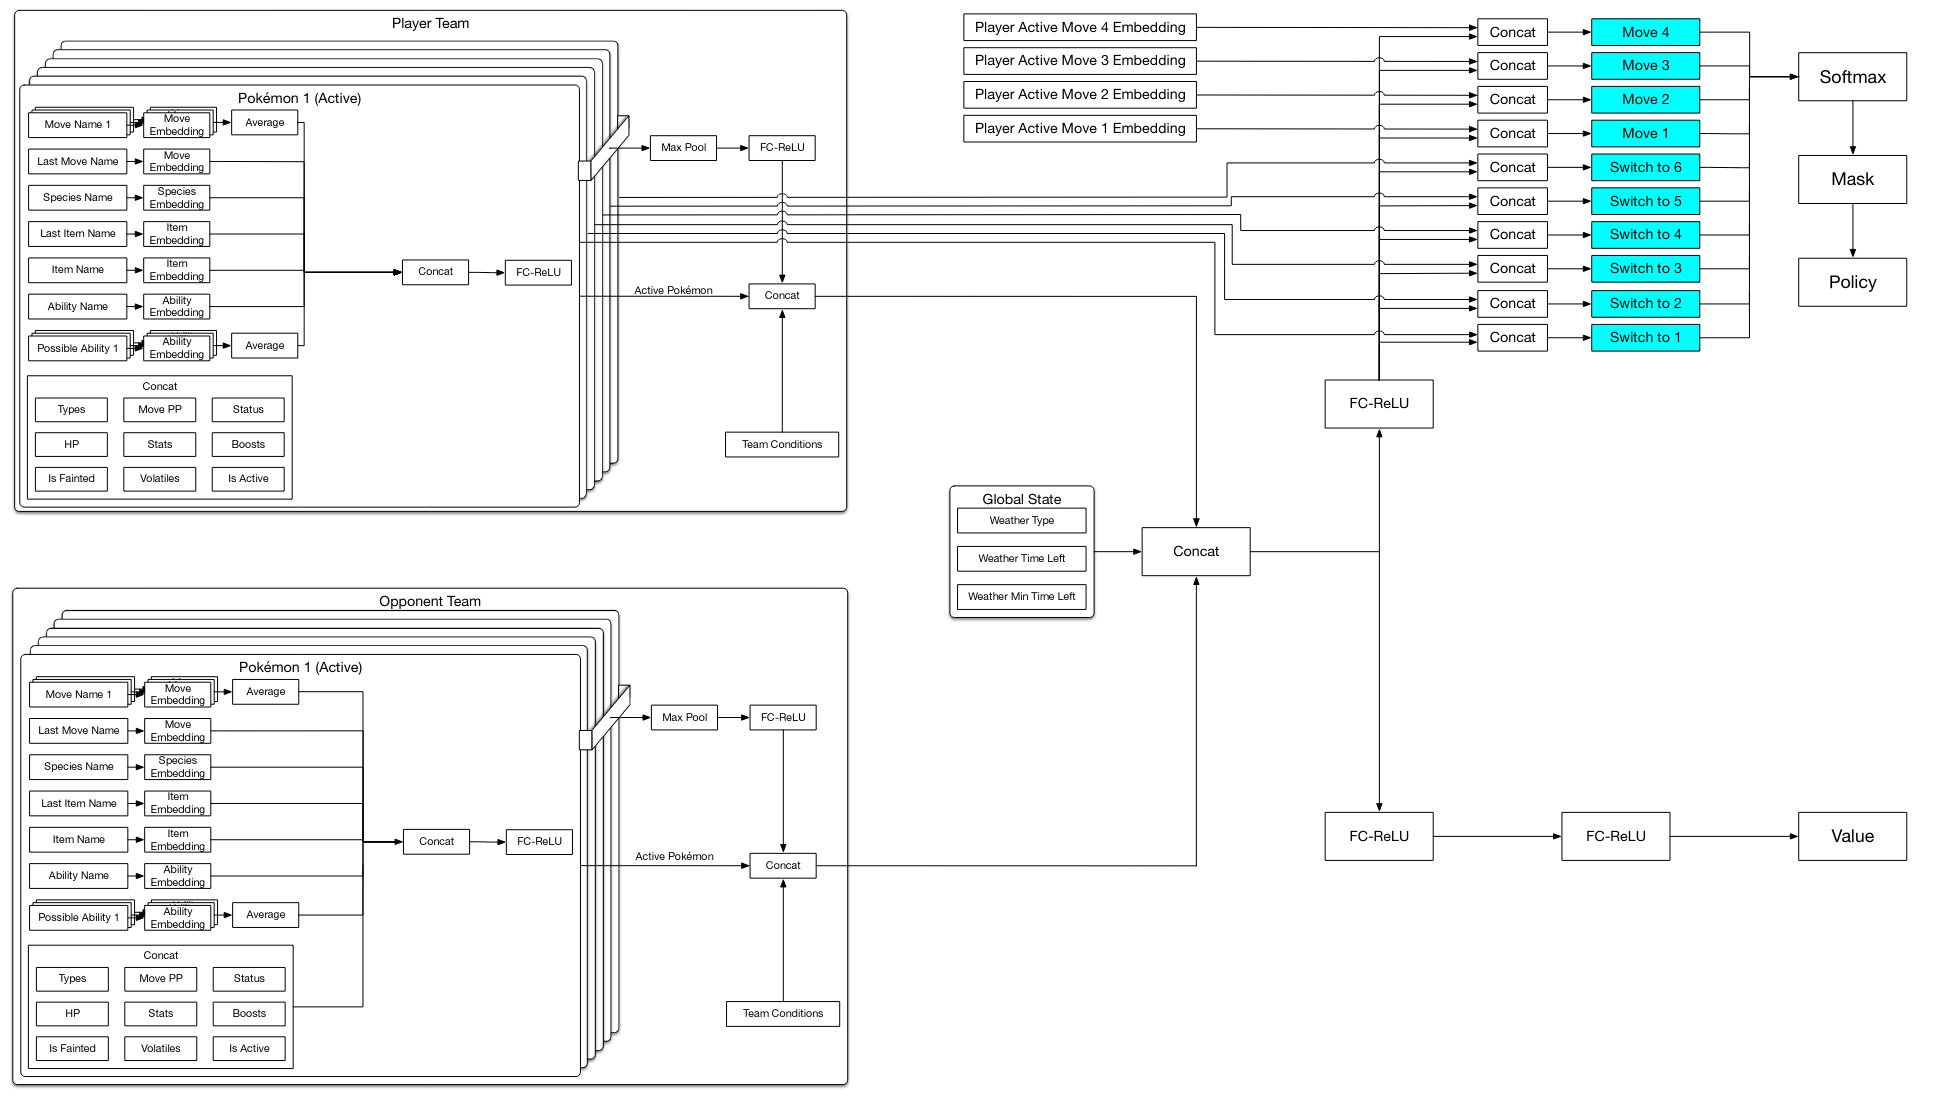
\includegraphics[width=1\textwidth]{images/RL-Network-Structure.png}
	\caption{The actor-critic neural network used by the authors in~\autocite{Huang_Lee_2019}}
	\label{fig:lee-network}
\end{sidewaysfigure}

\section{Approach}
\begin{sidewaysfigure}[h]
	\centering
	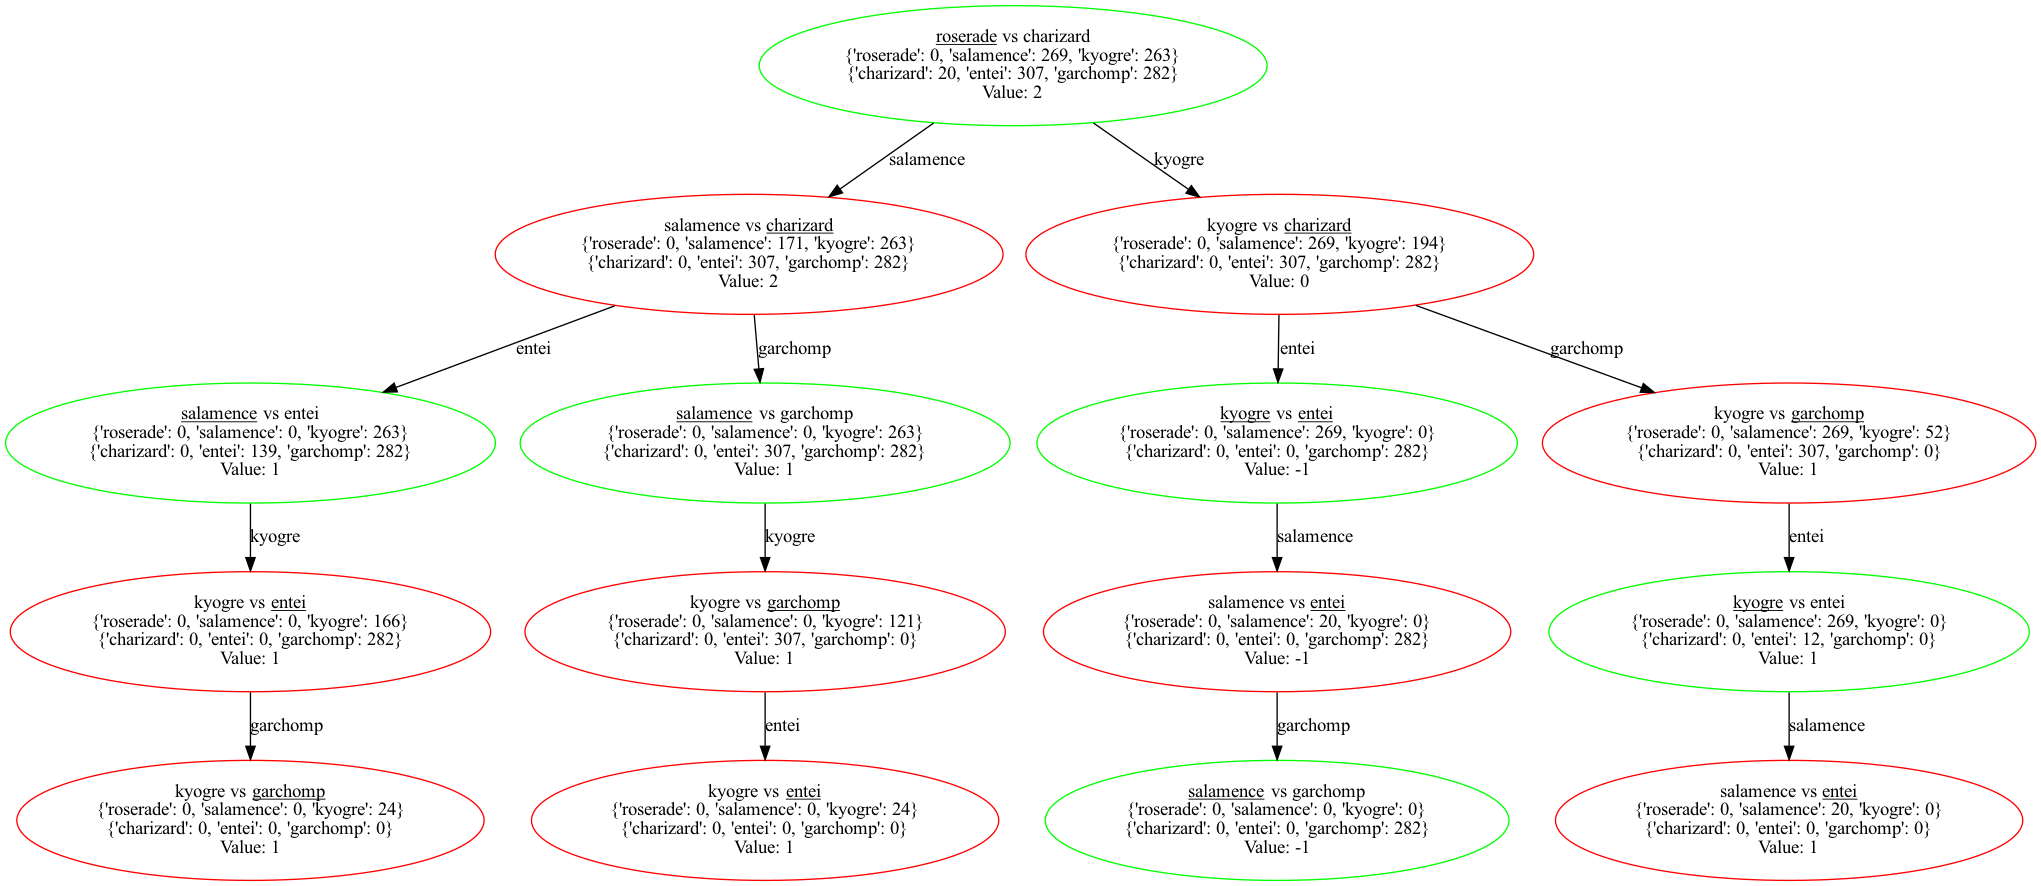
\includegraphics[width=1\textwidth]{images/MinMaxTree.png}
	\caption{Possible end game scenario}
	\label{fig:game-plan}
\end{sidewaysfigure}


